%----------------------------------------------------------------------------
%----------------------------------------------------------------------------
%bb defines the bounding box for the pdf
%viewport defines the area of the pdf used
%in sidewaysfigure the last entry in bb moves the caption toward/away the pic
%in sidewaysfigure the second entry in bb moves the pic toward/away the caption
%----------------------------------------------------------------------------
\begin{figure}
\scalebox{0.8}[0.8]{
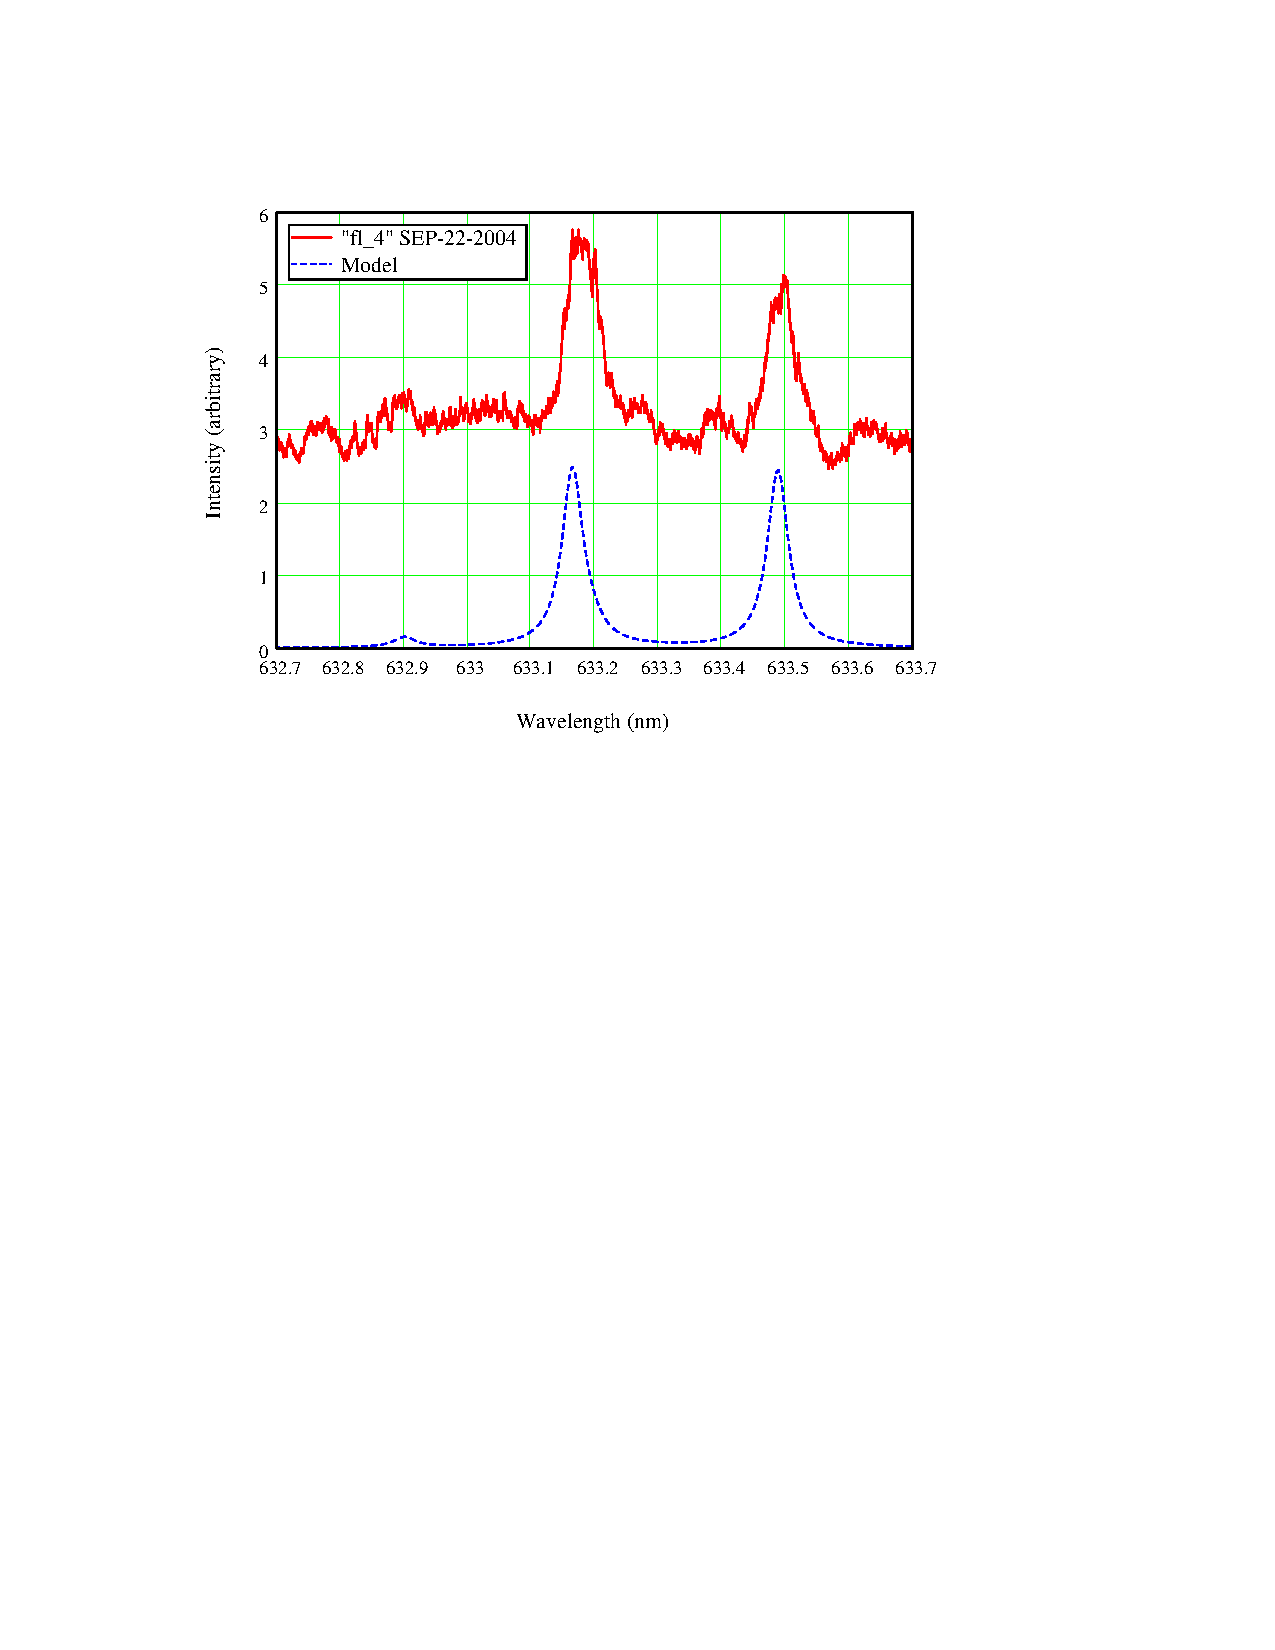
\includegraphics[bb=10 450 489 685]
{fl_4/fl_4.pdf}
}
\caption{535.8843 nm LIF (from ``transition one'')}
\label{fl_4}
\end{figure}
%----------------------------------------------------------------------------

%----------------------------------------------------------------------------
%bb defines the bounding box for the pdf
%viewport defines the area of the pdf used
%in sidewaysfigure the last entry in bb moves the caption toward/away the pic
%in sidewaysfigure the second entry in bb moves the pic toward/away the caption
%----------------------------------------------------------------------------
\begin{figure}
\scalebox{0.8}[0.8]{
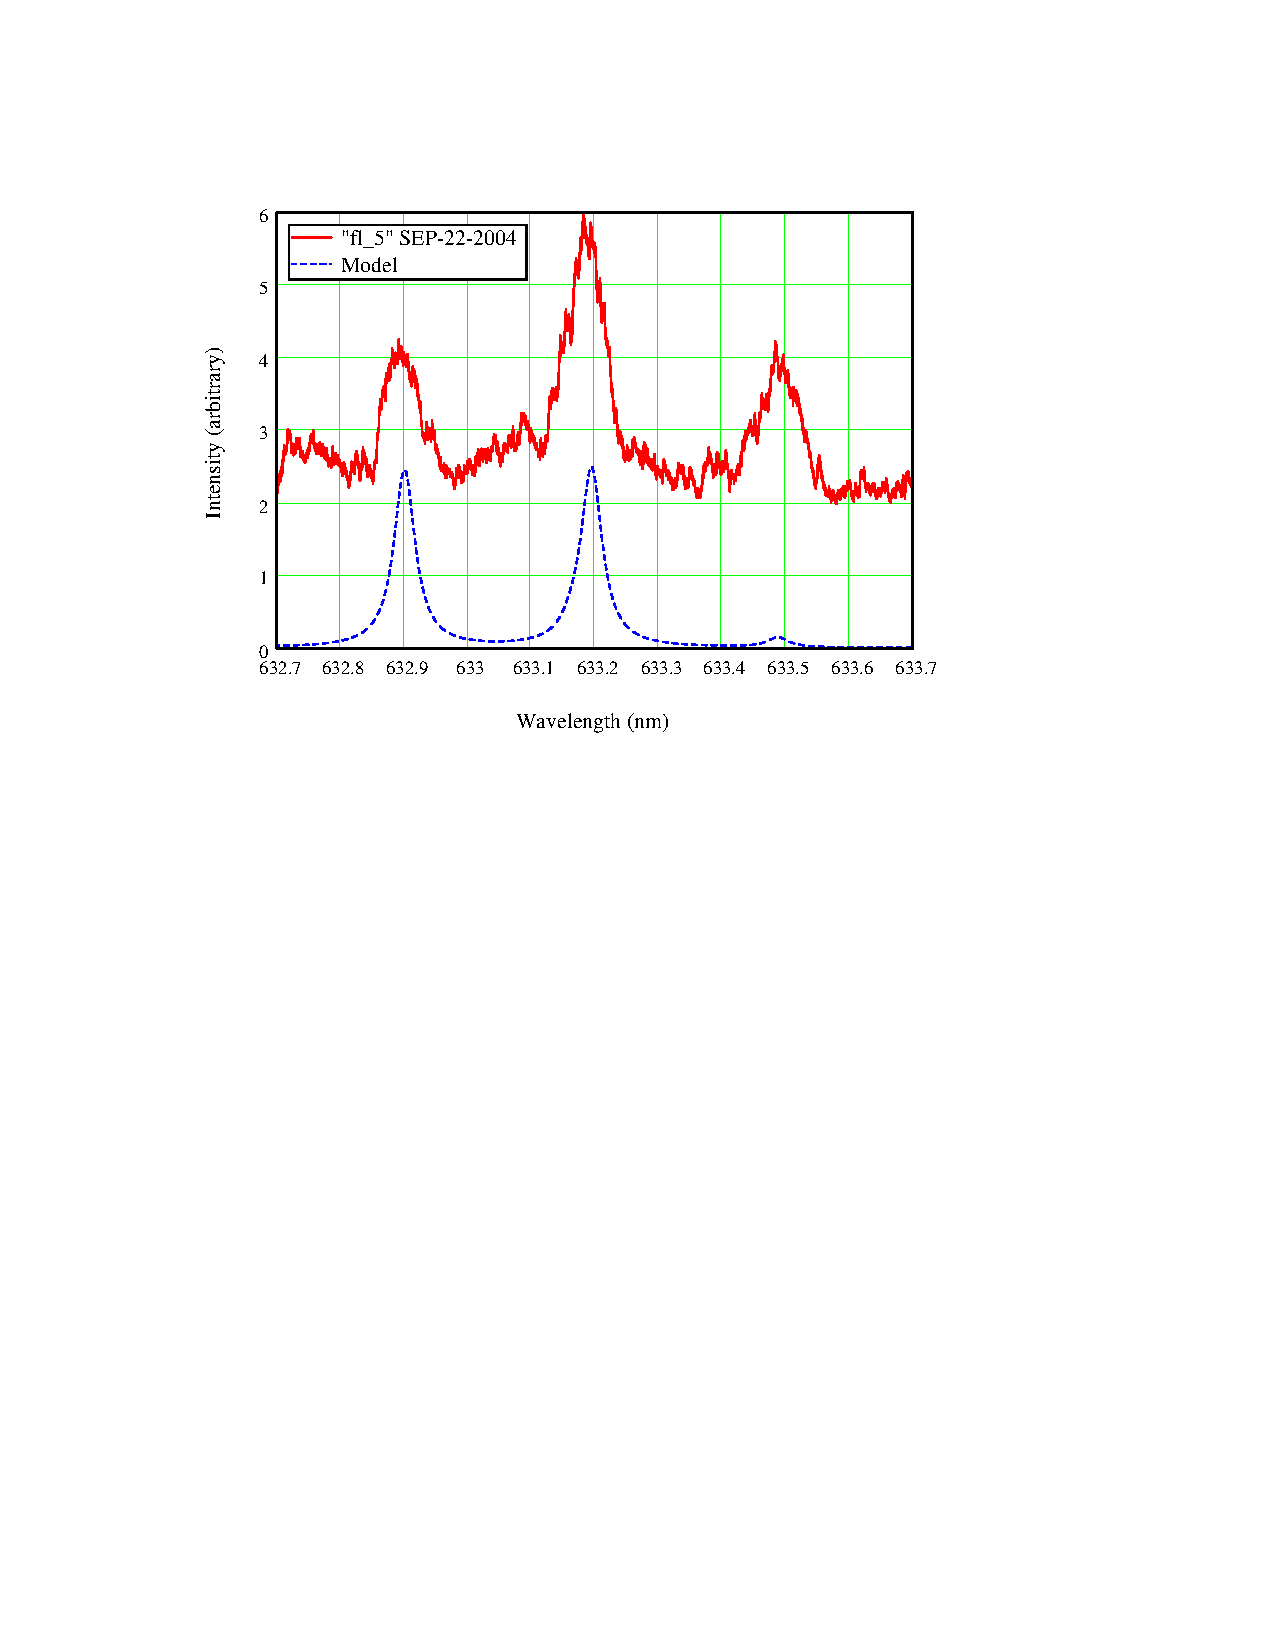
\includegraphics[bb=10 450 489 685]
{fl_5/fl_5.pdf}
}
\caption{535.8901 nm LIF (from ``transition two'')}
\label{fl_5}
\end{figure}
%----------------------------------------------------------------------------

%----------------------------------------------------------------------------
The fluorescence feature near 633 nm is shown in Figures \ref{fl_4} and \ref{fl_5}. The basic characteristics of the feature is its ``paired'' nature. Two lines representing the $J=\pm1$ transitions (see Section \ref{iodine levels section}) are clearly resolved in these data. The pair at 633.17 nm and 633.49 nm are associated with transition one (535.8843 nm). The pair at 632.90 nm and 633.20 nm are associated with transition two(535.8901 nm). See Figure \ref{fl_4} for the resulting features when the laser is tuned for 535.8843 nm and see Figure \ref{fl_5} for the resulting features when the laser is tuned for 535.8901 nm.

At first glance it seems that transition one was hit well and transition two was not. According to the model, the excited transitions (535.8843 nm and 535.8901 nm) should result in fluorescence with roughly the same intensity in the spectral window under consideration. Inspection of Figures \ref{fl_4} and \ref{fl_5} shows that the non-overlapped line (the right most line in Figure \ref{fl_4} and the left most line in Figure \ref{fl_5}) do not have the same heights. In fact the data plotted in Figure \ref{fl_5} are consistent with excitation somewhere between transition one and two. This may be the result of a 3-4 pm shift in the calibration of the dye laser and/or the ``lambdalok'' feature performing below specification. And, since these transitions are separated by 6 GHz, it indicates that selective excitation can be difficult due to the relatively broad dye laser spectrum.
%----------------------------------------------------------------------------
%----------------------------------------------------------------------------
%----------------------------------------------------------------------------
